%--------------------------------------------------------------------
\medskip
\subsection{Análisis funcional y diagrama de arquitectura de flujo de datos}
\label{02}
El sistema que se va a implementar consta de la siguiente funcionalidad:
\begin{itemize}
 \item Primero recogerá los datos del origen de datos (en este caso, del fichero CSV) y le aplicará técnicas ETL.
 \item Para posteriormente, formalizar un Data Mart con la información ya procesada.
 \item Se aplican herramientas OLAP para proporcionarle multidimensionalidad al Data Mart.
 \item Y así, permitir a los usuarios finales la posiblidad de realizar el análisis de las encuestas realizadas en todos los centros de sus clientes y poder hacer un seguimiento de los mismos.
\end{itemize}

Así pues, en la Figura \ref{02-image} se muestra la arquitectura del flujo de datos. 
\begin{figure}[!th]
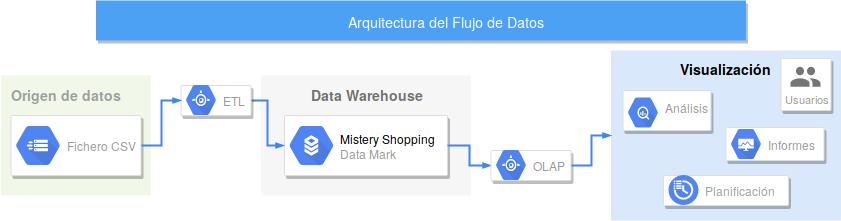
\includegraphics[scale=0.5]{02.png}
\centering
\caption{Arquitectura del flujo de datos}
\label{02-image}
\end{figure}
